% LaTeX header injected into the booklet build via pandoc
% --include-in-header. Drives the BTClock-orange link colour, the
% running headers/footers, and a few typographic niceties that are
% awkward to express via pandoc -V toggles.

\usepackage{xcolor}
\definecolor{BTOrange}{HTML}{E04300}
\definecolor{BTPanelGrey}{HTML}{DADBDE}
\definecolor{BTGold}{HTML}{D9AA2C}
\definecolor{BTDark}{HTML}{0A0A0A}

\usepackage{fancyhdr}
\pagestyle{fancy}
\fancyhf{}
\fancyhead[LE]{\textcolor{BTOrange}{\textbf{BTClock}} \textit{\nouppercase{\leftmark}}}
\fancyhead[RO]{\textit{\nouppercase{\rightmark}} \textcolor{BTOrange}{\textbf{BTClock}}}
\fancyfoot[LE,RO]{\thepage}
\renewcommand{\headrulewidth}{0.4pt}
\renewcommand{\headrule}{\hbox to\headwidth{\color{BTOrange}\leaders\hrule height \headrulewidth\hfill}}

\fancypagestyle{plain}{
  \fancyhf{}
  \fancyfoot[C]{\thepage}
  \renewcommand{\headrulewidth}{0pt}
}

% Tighten chapter spacing — A5 pages don't need the report class's
% generous default vertical lead-in.
\usepackage{titlesec}
\titleformat{\chapter}[display]
  {\normalfont\huge\bfseries\color{BTOrange}}
  {\chaptertitlename\ \thechapter}{14pt}{\Huge}
\titlespacing*{\chapter}{0pt}{-20pt}{20pt}

% Section / subsection use BTClock orange too.
\titleformat*{\section}{\Large\bfseries\color{BTOrange}}
\titleformat*{\subsection}{\large\bfseries\color{BTDark}}
\titleformat*{\subsubsection}{\normalsize\bfseries\color{BTDark}}

% Tables: alternate-row shading so dense feature/settings tables stay
% scannable at A5 size.
\usepackage{xcolor,colortbl}
\rowcolors{2}{BTPanelGrey!30}{white}

% Allow long URLs to break instead of overflowing the text block.
\usepackage{xurl}

% Emoji and other code points that the body font may not cover.
\usepackage{newunicodechar}
\newunicodechar{✅}{\textcolor{BTOrange}{\checkmark}}
\newunicodechar{❌}{\textcolor{BTOrange}{$\times$}}
\newunicodechar{⚠}{\textcolor{BTOrange}{!}}
\newunicodechar{➜}{$\rightarrow$}
\newunicodechar{→}{$\rightarrow$}
\newunicodechar{←}{$\leftarrow$}
\newunicodechar{↔}{$\leftrightarrow$}
\newunicodechar{·}{\textperiodcentered}
\newunicodechar{…}{\ldots}
\newunicodechar{≤}{$\leq$}
\newunicodechar{≥}{$\geq$}
\newunicodechar{²}{$^{2}$}
\newunicodechar{³}{$^{3}$}
% ₿ (BITCOIN SIGN, U+20BF) lives outside DejaVu Sans Mono's coverage;
% map it to a stylised B that reads correctly in body and code
% contexts. Real fix is bundling a Bitcoin glyph font, but this keeps
% the booklet building on a stock TeX install.
\newunicodechar{₿}{B\kern-0.55em\rule[0.04em]{0.06em}{0.95em}\kern0.45em}

% Cap image width to the text block so wide screen renders fit on the
% page; preserve aspect ratio.
\usepackage{graphicx}
\setkeys{Gin}{width=\linewidth,keepaspectratio}

% Pandoc emits `\begin{longtable}[]{@{}ll@{}}` for gfm tables without
% explicit column widths, and the image cells then render at native
% pixel size and overflow the text block. Detect the longtable
% context and shrink \pandocbounded so two-image-side-by-side tables
% (verticalDesc / invertedColor / suffix mode / etc.) and the
% three-column font-preview table both fit on the page.
\usepackage{etoolbox}
\usepackage{adjustbox}
\newif\ifBTinlongtable
\AtBeginEnvironment{longtable}{\BTinlongtabletrue}
\AtEndEnvironment{longtable}{\BTinlongtablefalse}
\AtBeginDocument{%
  \renewcommand{\pandocbounded}[1]{%
    \ifBTinlongtable
      \begin{adjustbox}{max size={0.46\linewidth}{0.5\textheight}}#1\end{adjustbox}%
    \else
      \begin{adjustbox}{max size={\linewidth}{0.85\textheight}}#1\end{adjustbox}%
    \fi
  }%
}

% Code blocks: subtle background panel, monospaced.
\usepackage{fancyvrb}
\fvset{frame=single,framerule=0pt,rulecolor=\color{BTPanelGrey},
       fontsize=\footnotesize}

% Wide / dense markdown tables on A4 sometimes overshoot the text
% block when pandoc emits explicit \real{} column widths. Force long
% tables to fit the page width and let cells wrap, and tighten the
% column padding so the hardware/settings tables breathe.
\usepackage{array}
\setlength{\tabcolsep}{4pt}
\renewcommand{\arraystretch}{1.15}
\AtBeginDocument{%
  \let\origlongtable\longtable
  \def\longtable{\setlength{\LTpre}{6pt}\setlength{\LTpost}{6pt}\origlongtable}%
}

% Custom cover page: full-bleed dark band, brand-orange title,
% subtitle, and a hero render of a BTClock screen. Replaces pandoc's
% default \maketitle which prints author/date we don't want. The
% wordmark uses Ubuntu Medium Italic to match the "BTClock" text
% engraved on the acrylic frame.
\usepackage{tikz}
\usetikzlibrary{positioning}
\usepackage{eso-pic}
\newfontfamily\BTCoverFont{Ubuntu Medium}[ItalicFont={Ubuntu Medium Italic}]
\renewcommand{\maketitle}{%
  \begin{titlepage}%
    \thispagestyle{empty}%
    \AddToShipoutPictureBG*{%
      \AtPageUpperLeft{%
        \tikz[remember picture,overlay]{%
          \fill[BTDark] (0,0) rectangle (\paperwidth,-0.42\paperheight);%
        }%
      }%
    }%
    \begin{center}%
      \vspace*{18mm}%
      {\color{white}\BTCoverFont\itshape\fontsize{72pt}{80pt}\selectfont BTClock\par}%
      \vspace{6mm}%
      {\color{BTOrange}\BTCoverFont\itshape\Large User \& developer handbook\par}%
      \vspace{2mm}%
      {\color{white}\BTCoverFont\itshape\large v4 firmware\par}%
      \vspace{30mm}%
      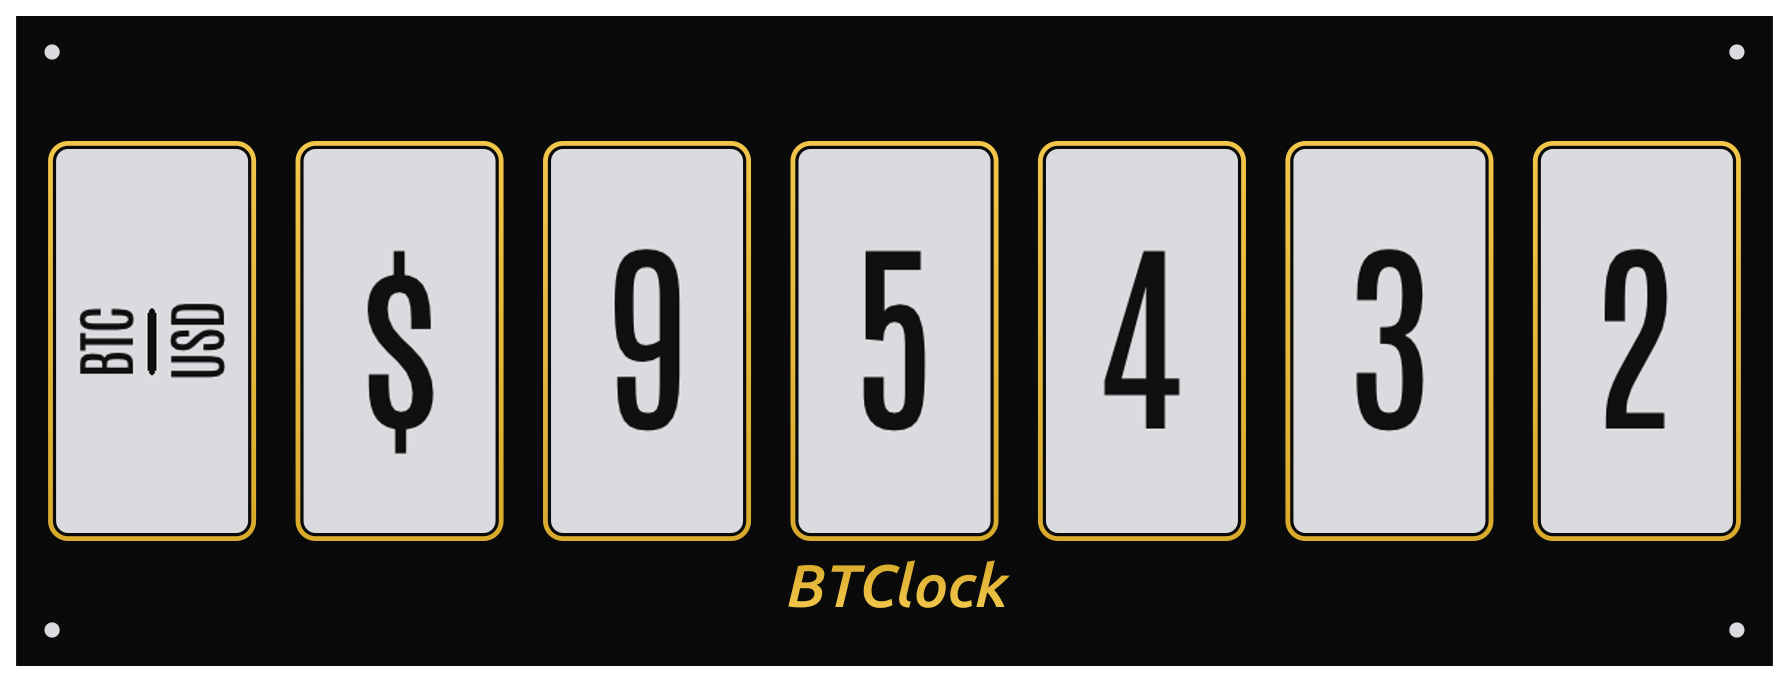
\includegraphics[width=0.92\linewidth]{docs/img/screens/btc_price.png}%
      \vfill%
      {\color{BTOrange}\rule{0.35\linewidth}{1pt}\par}%
      \vspace{4mm}%
      {\BTCoverFont\itshape\large btclock.dev\par}%
    \end{center}%
  \end{titlepage}%
  \cleardoublepage%
}
